\documentclass[12pt]{scrartcl}
\usepackage[sexy]{evan}
\usepackage{graphicx,amsmath,amssymb,amsthm,amsfonts,babel}
\usepackage{tikz, tkz-euclide}
\usepackage{lipsum}
\usepackage{setspace}
\graphicspath{ {./} }
\usetikzlibrary{calc,through,intersections}
\usepackage[paperwidth=16cm, paperheight=16cm,margin=0.8cm]{geometry}

\colorlet{EvanRed}{Red!50!Purple}

\newcommand{\siku}[4][.5cm]
	{
	\coordinate (tempa) at ($(#3)!#1!(#2)$);
	\coordinate (tempb) at ($(#3)!#1!(#4)$);
	\coordinate (tempc) at ($(tempa)!0.5!(tempb)$);%midpoint
	\draw[black] (tempa) -- ($(#3)!2!(tempc)$) -- (tempb);
	}
	\usetikzlibrary{calc,positioning,intersections}

\setstretch{1.5}

\usepackage{etoolbox}
\newcommand{\zerodisplayskips}{%
  \setlength{\abovedisplayskip}{5pt}%
  \setlength{\belowdisplayskip}{5pt}%
  \setlength{\abovedisplayshortskip}{5pt}%
  \setlength{\belowdisplayshortskip}{5pt}}
\appto{\normalsize}{\zerodisplayskips}
\appto{\small}{\zerodisplayskips}
\appto{\footnotesize}{\zerodisplayskips}
\setlength\parindent{10pt}

\title{International Mathematical Olympiad 2022 Problem 4}
\author{Solved by Azzam}
\date{This problem is too easy for IMO hehe}


\begin{document}
\maketitle
\pagestyle{plain}
\vspace{-1.5cm}

\newpage
\section{Soal}
\subsection{English}
Let $ABCDE$ be a convex pentagon such that $BC=DE$. Assume that there is a point $T$ inside $ABCDE$ with $TB=TD,TC=TE$ and $\angle ABT = \angle TEA$. Let line $AB$ intersect lines $CD$ and $CT$ at points $P$ and $Q$, respectively. Assume that the points $P,B,A,Q$ occur on their line in that order. Let line $AE$ intersect $CD$ and $DT$ at points $R$ and $S$, respectively. Assume that the points $R,E,A,S$ occur on their line in that order. Prove that the points $P,S,Q,R$ lie on a circle.

\subsection{Bahasa Indonesia}
Misalkan $ABCDE$ adalah sebuah segilima konveks sedemikian sehingga $BC=DE$. Asumsikan terdapat titik $T$ di dalam $ABCDE$ dengan $TB=TD,TC=TE$ dan $\angle ABT = \angle TEA$. Garis $AB$ memotong garis $CD$ dan $CT$ secara berturut-turut di titik $P$ dan $Q$. Titik-titik $P,B,A,Q$ berada di garis dengan urutan tersebut. Garis $AE$ memotong $CD$ dan $DT$ secara berturut-turut di titik $R$ and $S$. Titik-titik $R,E,A,S$ berada di garis dengan urutan tersebut. Buktikan bahwa titik-titik $P,S,Q,R$ berada di satu lingkaran yang sama.

\newpage
\section{Komentar}
Setelah melihat soal IMO tahun ini dan menyadari bahwa geometri ada di nomor 4 (nomor termudah di hari kedua), langsung kuputuskan untuk mencoba (because why not, easiest problem on day 2 right?).

Tapi setelah mencoba sekitar 15 menit dan nemu jawabannya, langsung saja aku kecewa, karena soalnya terasa lebih mudah daripada beberapa soal geometri yang diujikan di OSP bagian esai padahal ini setingkat IMO :/.

\newpage
\section{Solusi}
\begin{proof}[\textbf{Solusi.}]
Misalkan $M$ dan $L$ berturut-turut adalah perpotongan antara $RS$ dengan $QC$ dan $DS$ dengan $PQ$.

\begin{center}
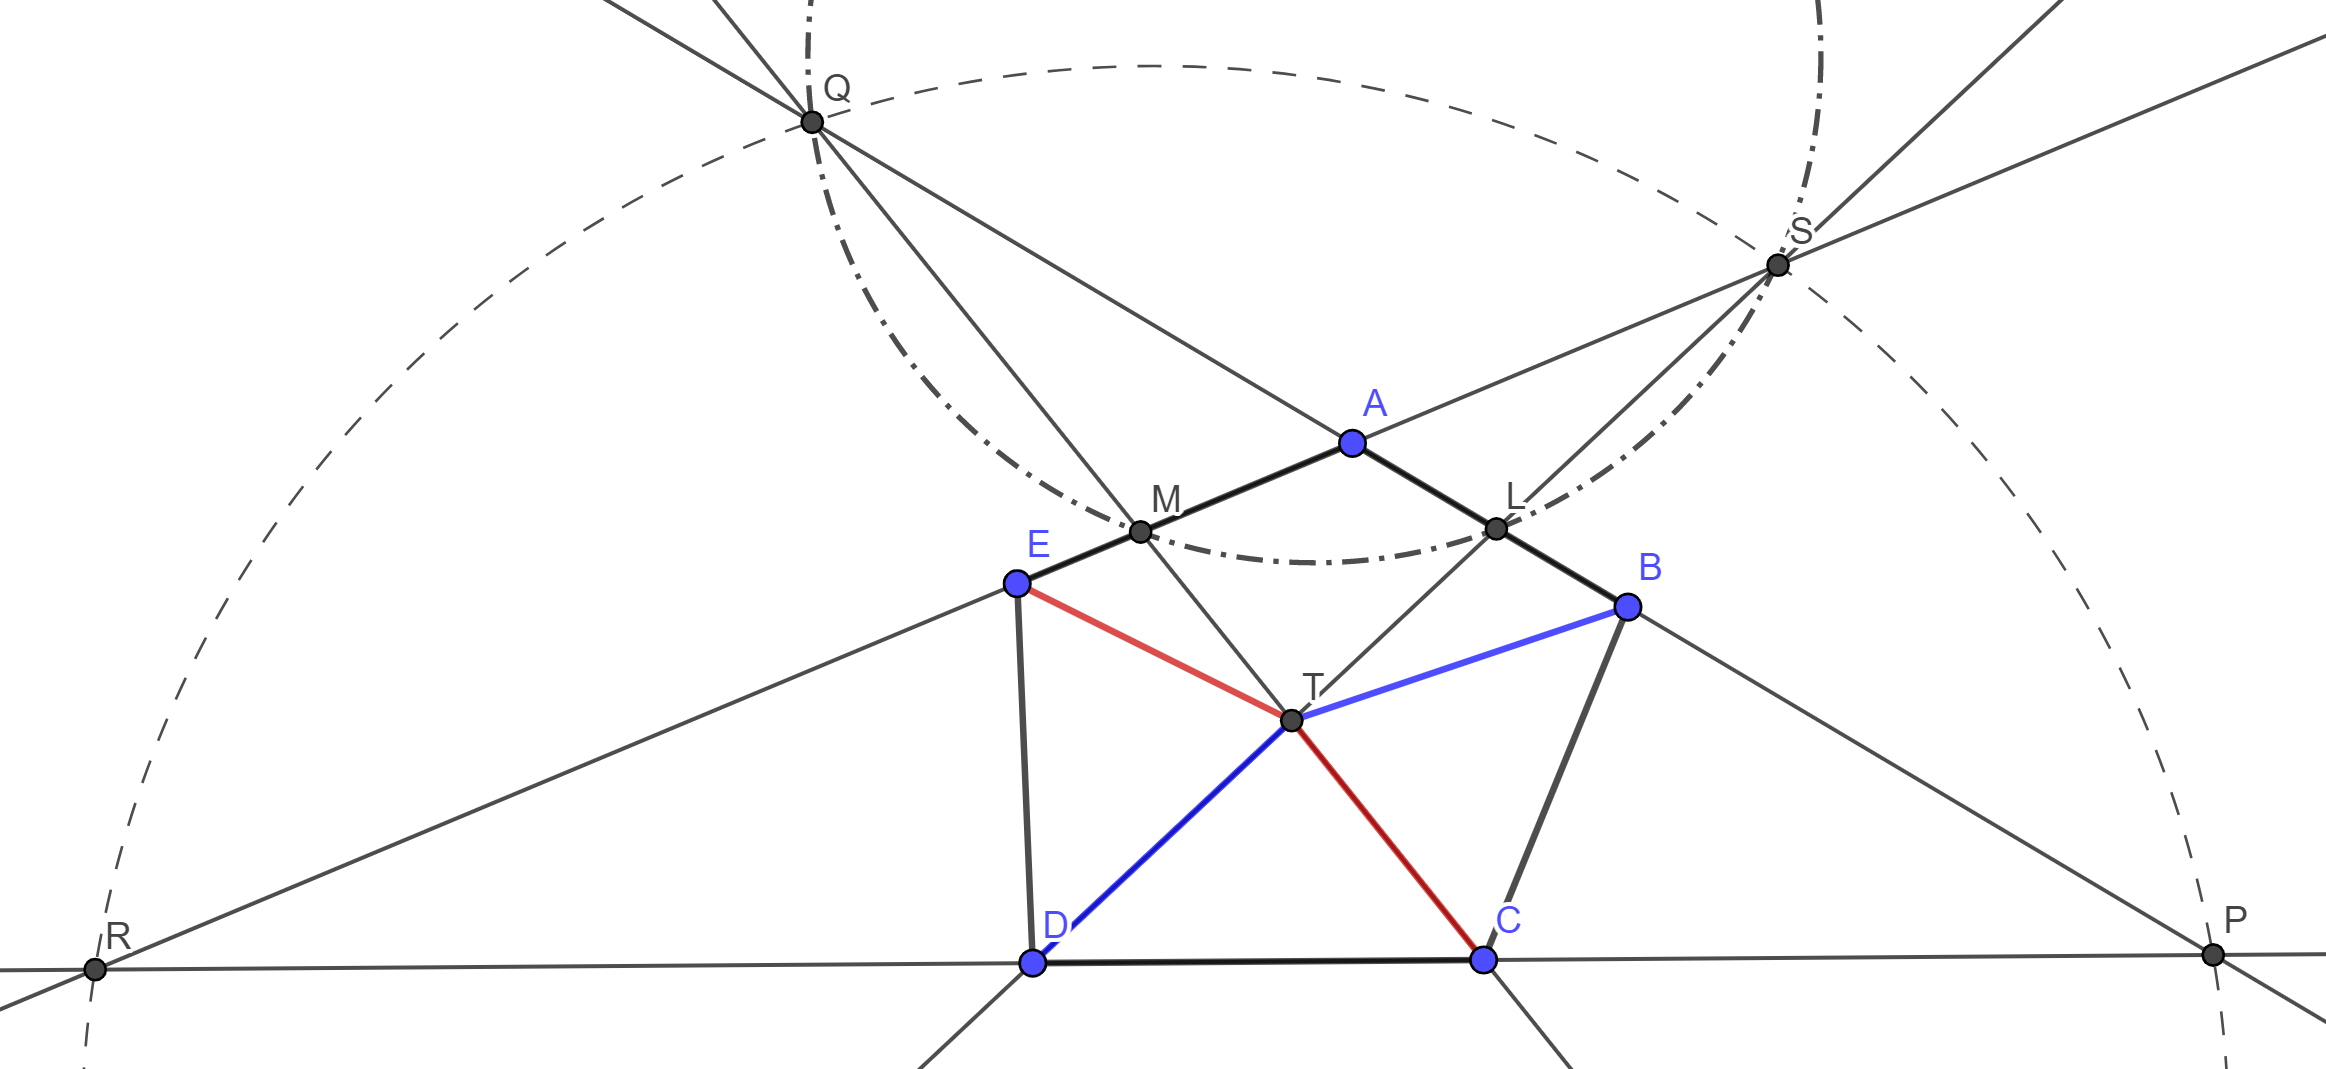
\includegraphics[scale=0.8]{p4.png}
\end{center}
Perhatikan karena $ET=TC$, $DT=TB$ dan $ED=CB$, maka didapat $\triangle ETD \cong \triangle CTB$ sehingga $\angle ETD = \angle CTB$.

Selanjutnya perhatikan bahwa
\begin{align*}
\angle MSL &= 180^\circ - \angle SET - \angle ETS \\
&= 180^\circ - \angle SET -(180^\circ-\angle ETD)\\
&= 180^\circ - \angle TBQ -(180^\circ-\angle CTB)\\
&= 180^\circ - \angle TBQ - \angle QTB\\
&= \angle MQL
\end{align*}
yang mengakibatkan $MQSL$ siklis. 

Selanjutnya, karena $\angle EST = \angle TQB$ dan $\angle TES = \angle QBT$, maka $\triangle BTQ \sim \triangle ETS$ sehingga dengan fakta $ET=TC$, $DT=TB$ juga, akan didapatkan
\begin{align}
\dfrac{ST}{TQ} = \dfrac{TE}{TB} = \dfrac{TC}{TD} \label{eq:1}
\end{align}

Namun, karena $MQSL$ siklis, kita punya $\angle MLT = 180^\circ - \angle MLS = \angle MQS = \angle TQS$. Selanjutnya, karena $\angle MTL = \angle STQ$ , maka $\triangle TML \sim \triangle STQ$ yang mengakibatkan
\begin{align}
\dfrac{TM}{TL} = \dfrac{TS}{TQ} \label{eq:2}
\end{align}
Oleh karena itu, dari $\eqref{eq:1}$ dan $\eqref{eq:2}$ didapatkan
\begin{align*}
\dfrac{TM}{TL} = \dfrac{TC}{TD} \implies ML \mid\mid CD \implies ML \mid\mid RP
\end{align*}
yang menyebabkan $\angle QLM = \angle QPR$.

Dari fakta $MQSL$ siklis dan fakta-fakta diatas akan didapatkan bahwa 
\begin{align*}
\angle QSR = \angle QSM = \angle QLM = \angle QPR
\end{align*}
yang menunjukkan bahwa $PSQR$ siklis. Terbukti.



\end{proof}
\end{document}